%%-*-latex-*-

% ------------------------------------------------------------------------
%
\begin{frame}
\frametitle{XML}

The acronym \XML stands for \textbf{eXtensible Markup Language}. It is
a language for defining unranked trees with plain text, such that the
syntax is easy to learn, write and understand, both for humans and
computer programs.

\bigskip

These trees are used to model \textbf{structured text documents}.

\bigskip

To understand what \XML is and how this modelling works, it is probably
easier to start with a small example.

\bigskip

Consider an e-mail. What are the different \textbf{elements} and what
is the \textbf{structure}, that is, how are the elements related to
each other?

\end{frame}

% ------------------------------------------------------------------------
%
\begin{frame}
\frametitle{XML/Example}

As far as the elements are concerned, an e-mail contains at least 
\begin{itemize}

  \item the recipient's address,

  \item a subject,

  \item the sender's address,

  \item a body of plain text.

\end{itemize}
The elements correspond to the tree nodes and the structure is modeled
by the shape of the tree itself.

\end{frame}

% ------------------------------------------------------------------------
%
\begin{frame}[containsverbatim]
\frametitle{XML/Example (cont)}

For example:

\bigskip

\noindent\rule{\linewidth}{0.5pt}
\begin{semiverbatim}
From: Me
Subject: Homeworks
To: You

  A \emph{deadline} is a due date for your \textbf{homework}.
\end{semiverbatim}
\rule{\linewidth}{0.5pt}

\end{frame}

% ------------------------------------------------------------------------
%
\begin{frame}
\frametitle{XML/Example (cont)}

This e-mail can be modeled by a tree as follows:
\begin{center}
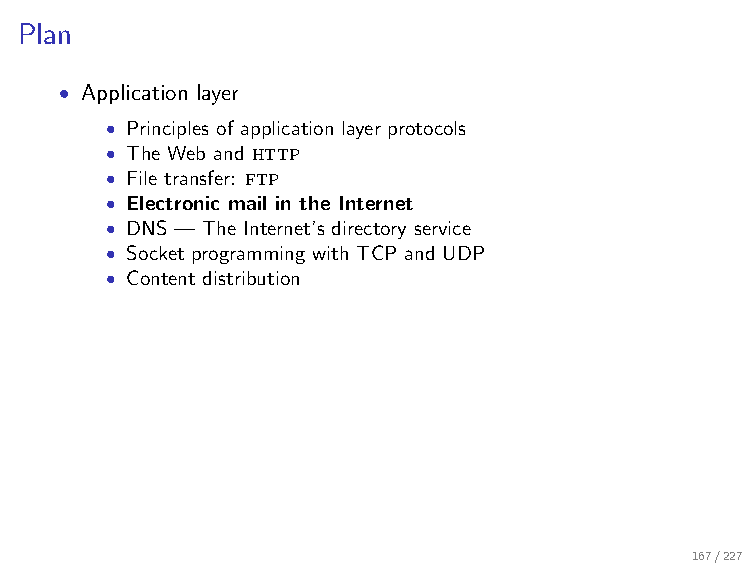
\includegraphics[scale=1,bb=71 624 385 721]{mail}
\end{center}
Notice that the (boxed) leaves contain text whereas the inner nodes
contain information \textbf{about} their subtrees, in particular the
leaves.

\end{frame}

% ------------------------------------------------------------------------
%
\begin{frame}[containsverbatim]
\frametitle{XML/Example (cont)}

Since the information of the inner nodes describes the information
actually laid out, it is called \textbf{meta-data} or
\textbf{mark-up}. The way to write this document in \XML is as
follows.
{\small
\begin{verbatim}
<mail>
  <from>Me</from>
  <subject>Homeworks</subject>
  <to>You</to>
  <body>
  A <definition>deadline</definition> is a due date for your
<emphasis>homework</emphasis>.
  </body>
</mail>
\end{verbatim}
}

\end{frame}

% ------------------------------------------------------------------------
%
\begin{frame}
\frametitle{XML/Tags}

Each subtree is denoted by an opening and a closing \textbf{tag}. An
opening tag is a name enclosed between \texttt{<} and \texttt{>}. A
closing tag is a name enclosed between \texttt{</} and \texttt{>}. 

\bigskip

The \textbf{tag name} is not part of the text, it is meta-data, so it
suggests the meaning of the data contained in the subtree.

\bigskip

For example, the whole \XML document is enclosed in tags whose name is
``\texttt{mail}'' because the document describes a mail.

\bigskip

Note the tag names ``\texttt{body}'', ``\texttt{definition}'' and
``\texttt{emphasis}'': this is the way we interpreted the red colour
and the italics in the mail, but other interpretations are possible:
such interpretations are \textbf{not} defined in \XML.

\end{frame}

% ------------------------------------------------------------------------
%
\begin{frame}[containsverbatim]
\frametitle{XML/Elements, nodes and declaration}

An \XML tree is called an \textbf{element} in \XML parlance. In
particular, the element including all the others is called the
\textbf{root element} (here, it is named ``\texttt{mail}'').

\bigskip

A node in the \XML tree corresponds, for now, to the opening and
closing tags only. The nodes have the same order as the elements.

\bigskip

The data (as opposed to the meta-data) is always contained in the
leaves, and is always text.

\bigskip

Our example is not exactly a correct \XML document because it lacks a
special element which says that the document is indeed \XML, and, more
precisely, what is the version of \XML used here, e.g.,
\begin{verbatim}
<?xml version="1.0"?>
\end{verbatim}

\end{frame}

% ------------------------------------------------------------------------
%
\begin{frame}[containsverbatim]
\frametitle{XML/Declaration and empty elements}

This special element is actually not an element, as the special
markers \texttt{<?} and \texttt{?>} tend to show. It is more a
declaration, some information about the current file, to destination
of the reader, whether it is a parsing software, usually called an
\textbf{\XML processor}, or a human.

\bigskip

Consider now the following element:
\begin{verbatim}
<axiom>
The empty set <empty/> contains no elements.
</axiom>
\end{verbatim}
which could be interpreted as\\

\noindent\rule{\linewidth}{0.5pt}
\textsf{
\textbf{Axiom}: The empty set \(\varnothing\) contains no elements. 
}\\

\noindent\rule{\linewidth}{0.5pt}

\end{frame}

% ------------------------------------------------------------------------
%
\begin{frame}[containsverbatim]
\frametitle{XML/Empty elements (cont)}

This \verb|<empty/>| is an \textbf{empty element}, it has a special
syntax for ending the tag, \verb|/>|, and it is neither an opening nor
a closing tag.

\bigskip

It is useful for denoting things, as symbols, that cannot be written
as text and need to be distinguished from text.
\begin{center}
\includegraphics[bb=71 680 306 721]{axiom}
\end{center}
An empty element corresponds to a leaf in the \XML tree, despite it is
meta-data data and not data.

\end{frame}

% ------------------------------------------------------------------------
%
\begin{frame}[containsverbatim]
\frametitle{XML/Repeated nodes}

Nodes do not need to be unique at a given tree level. For instance, if
we want to send a mail to several recipients we would write:
{\small
\begin{semiverbatim}
<mail>
  <from>Me</from>
  <subject>Homeworks</subject>
  <to>You</to>
  \textbf{<to>Me</to>} 
  <body>
  A <definition>deadline</definition> is a due date for your
<emphasis>homework</emphasis>.
  </body>
</mail>
\end{semiverbatim}
}

\end{frame}

% ------------------------------------------------------------------------
%
\begin{frame}
\frametitle{XML/Repeated nodes (cont)}

The \XML tree associated to this \XML document is
\begin{center}
\includegraphics[bb=71 624 412 721,scale=0.9]{mailtoto}
\end{center}
Note that there are two nodes ``to'' at the same level, and that their
order must be the same as in the \XML document.

\end{frame}

% ------------------------------------------------------------------------
%
\begin{frame}[containsverbatim]
\frametitle{XML/Attributes}

It is possible to annotate each meta-data node with some labeled
strings, called \textbf{attributes}. For example, we may want to
specify that our mail is urgent, which is a property of the mail
as a whole, not a part of the contents per se:
{\small
\begin{semiverbatim}
<mail \textbf{priority="urgent"}>
  <from>Me</from>
  <subject>Homeworks</subject>
  <to>You</to>
  <body>
  A <definition>deadline</definition> is a due date for your
<emphasis>homework</emphasis>.
  </body>
</mail>
\end{semiverbatim}
}

\end{frame}

% ------------------------------------------------------------------------
%
\begin{frame}
\frametitle{XML/Attributes (cont)}

It is possible to represent that \XML document by the annotated tree
\begin{center}
\includegraphics[bb=71 623 386 721]{urgent}
\end{center}

\end{frame}

% ------------------------------------------------------------------------
%
\begin{frame}[containsverbatim]
\frametitle{XML/Attributes (cont)}

It is possible to attach several attributes to a given element, like
{\small
\begin{semiverbatim}
<mail \textbf{priority="urgent"} \textbf{ack="yes"}>
  <from>Me</from>
  <subject>Homeworks</subject>
  <to>You</to>
  <body>
  A <definition>deadline</definition> is a due date for your
<emphasis>homework</emphasis>.
  </body>
</mail>
\end{semiverbatim}
}
The order of the attributes matters. Any element can have attributes,
including empty elements.

\end{frame}

% ------------------------------------------------------------------------
%
\begin{frame}
\frametitle{XML/Attributes (cont)}

Attributes are considered to be a special kind of node, although they
are not often represented as such for room's sake.
\begin{center}
\includegraphics[bb=71 652 365 721]{attr}
\end{center}
Note the symbol \textsf{@} preceding the attribute name, which
distinguishes it from element nodes. At a given tree level, the
attribute nodes are placed \emph{before} the element nodes.

\end{frame}

% ------------------------------------------------------------------------
%
\begin{frame}[containsverbatim]
\frametitle{XML/Attributes (cont)}

The declaration can hold several attributes, besides
\verb|version|, like
\begin{verbatim}
<?xml version="1.0" encoding="UTF-8"?>
<?xml version='1.1' encoding="US-ASCII"?>
<?xml version= '1.0' encoding='iso-8859-1'?>
\end{verbatim}
The encoding is the \textbf{character encoding} of the \XML document,
which is particularly useful when using \Unicode or some Asian
fonts. 

\bigskip

Note that the attributes must be in lowercase, the \emph{value} of the
attributes can be enclosed in single or double quotes. 

\bigskip

In the case of \verb|version| and \verb|encoding|, only some
standardized values are valid.

\end{frame}

% ------------------------------------------------------------------------
%
\begin{frame}[containsverbatim]
\frametitle{XML/Escaping characters}

All programming languages offer strings of characters to the
programmer to use. For instance, in \Clang, the strings are enclosed
between double quotes: \verb|"abc"|. 

\bigskip

Thus, if the string contains double-quotes, we must take care of
\textbf{escaping} them, so the compiler (more precisely: the parser)
can distinguish the double-quotes in the contents from the enclosing
double-quotes. 

\bigskip

In \Clang, character escaping is achieved by adding a backslash just
before the character, e.g., \verb|"He said: \"Hello!\"."| is a valid
\Clang string.

\bigskip

In \XML, there is a similar problem. The attribute values can either
be enclosed by single or double quotes. If the latter, the
double-quotes in the contents need escaping; if the former, the quotes
need escaping. Problems also stem from the characters used for the
mark-up.

\end{frame}

% ------------------------------------------------------------------------
%
\begin{frame}[containsverbatim]
\frametitle{XML/Escaping characters (cont)}

For example, the following element
{\small
\begin{verbatim}
<problem>For all integer n, we have n < n + 1.</problem>
\end{verbatim}
}
is not valid because the text between the tags contains the character
``\texttt{<}'', which is confused by the \XML parsers with the (expected)
start of a tag:
{\small
\begin{semiverbatim}
<problem>For all integer n, we have n \textbf{<} n + 1.</problem>
\end{semiverbatim}
} 
The \XML way to escape this character is to use instead the special
sequence of characters \verb|&lt;| so the previous, corrected, element
becomes
{\small
\begin{semiverbatim}
<valid>For all integer n, we have n \textbf{&lt;} n + 1.</valid>
\end{semiverbatim}
}

\end{frame}

% ------------------------------------------------------------------------
%
\begin{frame}[containsverbatim]
\frametitle{XML/Predefined named entities}

The sequence \verb|&lt;| is called a \textbf{predefined named entity}.

\bigskip

Such entities always 
\begin{enumerate}
 
  \item start with an ampersand (\verb|&|), 

  \item continue with a predefined name (here, \texttt{lt}),

  \item end with a semi-colon (\texttt{;}).

\end{enumerate}
The choice of the ampersand to mark the start of a predefined named
entity entails that this very character must itself be escaped...

\bigskip

So one must always use \verb|&amp;| instead.

\end{frame}

% ------------------------------------------------------------------------
%
\begin{frame}[containsverbatim]
\frametitle{XML/Predefined named entities (cont)}

There are some other characters which can \emph{sometimes} cause a
problem to \XML parsers (as opposed to always create a problem, as
\verb|<| and \verb|&| do). 

\bigskip

A summary of all the predefined named entities is given in the
following table.
\begin{center}
\begin{tabular}{cll}
\toprule
Character & Entity & Mandatory\\
\midrule
\verb|&| & \verb|&amp;|  & always\\
\verb|<| & \verb|&lt;|   & always\\
\verb|>| & \verb|&gt;|   & in attribute values\\
\verb|"| & \verb|&quot;| & in double-quoted strings\\
\verb|'| & \verb|&apos;| & in single-quoted strings\\
\bottomrule
\end{tabular}
\end{center}

\end{frame}

% ------------------------------------------------------------------------
%
\begin{frame}
\frametitle{XML/Predefined named entities (cont)}

Consider
\footXMLin{entities.xml}

\end{frame}

% ------------------------------------------------------------------------
%
\begin{frame}[containsverbatim]
\frametitle{XML/Predefined numbered entities}

The two last entities are \textbf{predefined numbered entities} because
they denote characters by using their \Unicode code (which ranges from
\(0\) to \(65,536\)). 

\bigskip

Check out \url{http://www.unicode.org/} for \Unicode.

\bigskip

If the code is given in decimal (i.e., using base \(10\)), it is
introduced by \verb|&#|, e,g, \verb|&#100|.

\bigskip

If the code is given in hexadecimal (i.e., using base \(16\)), it is
introduced by \verb|&#x|, e.g., \verb|&#x00E7|.

\end{frame}

% ------------------------------------------------------------------------
%
\begin{frame}[containsverbatim]
\frametitle{XML/User-defined internal entities and document type declarations}

It can be annoying to use numbers to refer to characters, especially
if one considers that \Unicode requires four digits.

\bigskip

To make life easier, it is possible to bind a name to an entity
representing a character: a \textbf{user-defined internal entity}.

\bigskip

They are called internal because their definition must be in the same
document where they are used.

\end{frame}


% ------------------------------------------------------------------------
%
\begin{frame}[containsverbatim]
\frametitle{XML/User-defined internal entities and document type declarations (cont)}

For example, it is easier to use \verb|&n;| instead of \verb|&#241|,
especially if the text is in Spanish (this represents the letter
\texttt{\~{n}}).

\bigskip

This kind of entity must be declared in the \textbf{document type
declaration}, which is located, if any, just after the declaration
\verb|<?xml ... ?>| and before the root element.

\end{frame}

% ------------------------------------------------------------------------
%
\begin{frame}[containsverbatim]
\frametitle{XML/User-defined internal entities and document type declarations
  (cont)}
\label{xml_intro:DOCTYPE}

A document type declaration is made, from left to right, of
\begin{enumerate}

  \item an opening tag \verb|<!DOCTYPE|,

  \item the root element name,

  \item the character \verb|[|,
  
  \item the named character entity declarations,

  \item the closing tag \verb|]>|

\end{enumerate}

\end{frame}

% ------------------------------------------------------------------------
%
\begin{frame}[containsverbatim]
\frametitle{XML/User-defined internal entities and document type declarations (cont)}

A named character entity declaration is made, from left to right, of
\begin{enumerate}

  \item the opening tag \verb|<!ENTITY|,

  \item the entity name,

  \item the numbered character entity between double-quotes,

  \item the closing tag \verb|>|

\end{enumerate}
For example:
\begin{verbatim}
<!ENTITY n "&#241;">
\end{verbatim}

\end{frame}

% ------------------------------------------------------------------------
%
\begin{frame}
\frametitle{XML/User-defined internal entities and document type declarations (cont)}

A complete example:
\XMLin{espana.xml}
One can think such an entity as being a macro in \Cpp, the \Clang
preprocessor language.

\end{frame}

% ------------------------------------------------------------------------
%
\begin{frame}[containsverbatim]
\frametitle{XML/User-defined internal entities and document type declarations (cont)}

It is possible to extend user-defined internal entities to denote any
character string, not just a single character.

\bigskip

Typically, if one wishes to repeat a piece of text, like a company
name or a person's name, a good idea is to give a name to this string
and, wherever one want its contents, an entity with the given name is
put instead.

\bigskip

The syntax for the declaration is the same, but more characters are
put between double-quotes. For example,
\begin{verbatim}
<!ENTITY univ "Konkuk University">
<!ENTITY motto "<spain>Viva Espa&n;a!</spain>">
<!ENTITY n "&#241;">
\end{verbatim}

\end{frame}

% ------------------------------------------------------------------------
%
\begin{frame}[containsverbatim]
\frametitle{XML/External entities}

Sometimes the \XML document needs to include other \XML documents and
copying the external documents once is not a good strategy, since this
avoids keeping track of the evolution of these external documents.

\bigskip

Fortunately, \XML allows to specify the inclusion of other \XML
documents by means of \textbf{external entities}. The declaration of
these entities is as follows:
\begin{enumerate}

  \item an opening tag \verb|<!ENTITY|,

  \item the entity name,

  \item the keyword \verb|SYSTEM|,

  \item the full name of the \XML file between double-quotes,

  \item the closing tag \verb|>|

\end{enumerate}

\end{frame}

% ------------------------------------------------------------------------
%
\begin{frame}[containsverbatim]
\frametitle{XML/External entities (cont)}

For example,
\begin{verbatim}
<?xml version="1.0"?>
<!DOCTYPE longdoc [
  <!ENTITY part1 SYSTEM "p1.xml">
  <!ENTITY part2 SYSTEM "p2.xml">
  <!ENTITY part3 SYSTEM "p3.xml">
]>
<longdoc>
  The included files are:
  &part1;
  &part2;
  &part3;
</longdoc>
\end{verbatim}

\end{frame}

% ------------------------------------------------------------------------
%
\begin{frame}[containsverbatim]
\frametitle{XML/External entities (cont)}

At parsing time, the external entities are fetched and copied into the
main \XML document, replacing the entity.

\bigskip

Therefore the included parts cannot contain any prolog, i.e., the \XML
declaration \verb|<?xml ... ?>| and the document type declaration
\verb|<!DOCTYPE ... ]>|, if any.

\bigskip

\XML processors are required, when reading an external entity, to copy
verbatim the content of the referred external document, and then parse
it as if it always belonged to the master document (that is, the one
which imports the others).

\end{frame}

% ------------------------------------------------------------------------
%
\begin{frame}[containsverbatim]
\frametitle{XML/Unparsed entities and notations}

\textbf{Unparsed entities} allow to refer to a binary objects, like
images, or some text which is not \XML, like a program. They are
declared by
\begin{enumerate}

  \item the opening tag \verb|<!ENTITY|,

  \item the entity name,

  \item the keyword \verb|SYSTEM|,

  \item the full name of the non-\XML external file between
    double-quotes,

  \item the keyword \verb|NDATA|,

  \item a notation (the kind of the file),

  \item the closing tag \verb|>|

\end{enumerate}

\end{frame}

% ------------------------------------------------------------------------
%
\begin{frame}
\frametitle{XML/Unparsed entities and notations (cont)}

Had we used external entities, the included object had been copied in
place of the reference and parsed as \XML{} ---~which it is
not. Consider
\smallXMLin{notation.xml}

\end{frame}

% ------------------------------------------------------------------------
%
\begin{frame}[containsverbatim]
\frametitle{XML/Unparsed entities and notations (cont)}

Notice the notation ``\texttt{gif}'', which is the kind of the
unparsed entity. Notations must be defined in the document type
declarations as
\begin{enumerate}

  \item the opening tag \verb|<!NOTATION|,

  \item the notation name,

  \item the keyword \verb|SYSTEM|,

  \item a description of the kind of unparsed entity the notation
    refers to (it can be a \MIME type, an URL, plain English...)

  \item the closing tag \verb|>|

\end{enumerate}

\end{frame}

% ------------------------------------------------------------------------
%
\begin{frame}
\frametitle{XML/Unparsed entities and notations (cont)}

Notice also that unparsed entities
\begin{itemize}

  \item must be used as attribute values (in our example, the
    attribute name is ``\texttt{image}''),

  \item are names (``\texttt{picture}''), instead of the usual entity
    syntax (``\texttt{\&picture;}'').

\end{itemize}

\end{frame}

% ------------------------------------------------------------------------
%
\begin{frame}[containsverbatim]
\frametitle{XML/Unparsed entities and notations (cont)}

This example is \textbf{not} well-formed.
\begin{verbatim}
<?xml version="1.0"?>
<!DOCTYPE doc [
  <!NOTATION jpeg SYSTEM "image/jpeg">
  <!ENTITY pic "pictures/me.jpeg" NDATA jpeg>
]>
<doc>
  &pic;
</doc>
\end{verbatim}

\end{frame}

% ------------------------------------------------------------------------
%
\begin{frame}
\frametitle{XML/A summary of all kinds of entities}

\begin{center}
\includegraphics[bb=71 627 276 721]{entities}
\end{center}

\end{frame}

% ------------------------------------------------------------------------
%
\begin{frame}[containsverbatim]
\frametitle{XML/Unparsed character data}

It is sometimes tiresome to have to escape characters, i.e., use
character entities.

\bigskip

To avoid the need of escaping, there is a special construct:
\textbf{CDATA sections} (short for ``Character DATA''), made of
\begin{enumerate}

  \item an opening tag \verb|<!CDATA[|,

  \item some text without escaping and without the sequence \verb|]]>|,

  \item a closing tag \verb|]]>|.

\end{enumerate}
For example 
\begin{semiverbatim}
<para>A test in C:
  <c>\textbf{<!CDATA[}if (x < y) return &r;\textbf{]]>}</c>
</para>
\end{semiverbatim}

\end{frame}

% ------------------------------------------------------------------------
%
\begin{frame}
\frametitle{XML/Internal linking}

Consider a document representing a technical book, like a textbook. It
is common to find cross-references in such kind of books, i.e.,
references in some chapters to other chapters or sections, or
bibliographical entries.

\bigskip

One easy way to achieve this is to use some attributes as labels and
some attributes as references.

\bigskip

The problem is that the writer is then in charge of checking whether 
\begin{itemize}

  \item a given label is unique in the whole document,

  \item every reference is linked to a label.

\end{itemize}

\end{frame}

% ------------------------------------------------------------------------
%
\begin{frame}
\frametitle{XML/Internal linking (cont)}
\label{xml_intro:ATTLIST}

\XML provides a way to ensure that any validating parser will check
this kind of internal linking automatically: using \texttt{ID} and
\texttt{IDREF}. 

\bigskip

The former is the kind of all the (attribute) labels and the latter is
the kind of all the (attribute) references.

\bigskip

The attributes used either as label or reference must be declared in
the \texttt{DOCTYPE} section using \texttt{ATTLIST}. 

\end{frame}

% ------------------------------------------------------------------------
%
\begin{frame}[containsverbatim]
\frametitle{XML/Internal linking/Labels}

For the labels, use
\begin{enumerate}

  \item an opening tag \verb|<!ATTLIST|,

  \item the name of the element being labelled,

  \item the names of the label attributes separated by spaces,

  \item the keyword \texttt{ID},

  \item the keyword \texttt{\#REQUIRED} if the element must always be
    labelled, otherwise \texttt{\#IMPLIED},

  \item a closing tag \verb|>|

\end{enumerate}

\end{frame}

% ------------------------------------------------------------------------
%
\begin{frame}[containsverbatim]
\frametitle{XML/Internal linking/References}

For the references, use
\begin{enumerate}

  \item an opening tag \verb|<!ATTLIST|,

  \item the name of the referring element,

  \item the names of the reference attributes separated by spaces,

  \item the keyword \texttt{IDREF},

  \item the keyword \texttt{\#REQUIRED} if the element must always
    carry a reference, otherwise \texttt{\#IMPLIED},

  \item a closing tag \verb|>|

\end{enumerate}

\end{frame}

% ------------------------------------------------------------------------
%
\begin{frame}
\frametitle{XML/Internal linking (cont)}
\label{xml_intro:id_idref}

For example,
\smallXMLin{id_idref.xml}

\end{frame}

% ------------------------------------------------------------------------
%
\begin{frame}[containsverbatim]
\frametitle{XML/Comments}

It is possible to include comments in an \XML document. They are made
of
\begin{enumerate}

  \item an opening tag ``\verb|<!--|'',

  \item some text without the sequence ``\verb|--|'',

  \item a closing tag ``\verb|-->|''.

\end{enumerate}
For example
{\small
\begin{semiverbatim}
<p>Our store is located at</p>
\textbf{<!--} <address>Eunpyeong-gu, Seoul</address> \textbf{-->}
<address>Gangnam-gu, Seoul</address>
\end{semiverbatim}
}
Contrary to programming languages, comments are \textbf{not} ignored
by the parsers and are nodes of the \XML tree.

\end{frame}

% ------------------------------------------------------------------------
%
\begin{frame}
\frametitle{XML/Namespaces}

Each \XML document defines its own element tags, we can call its
\emph{vocabulary}. 

\bigskip

In case we use external entities which refer to other \XML document
using, by coincidence, the same tags, we end with an ambiguity in the
master document.

\bigskip

A good way to avoid these name clashes it to use
\textbf{namespaces}. A namespace is a user-defined annotation of each
element tag names and attribute names.

\bigskip

Therefore, if two \XML documents use two different namespaces, i.e.,
two different tag annotations, there is no way to mix their elements
when importing one document into the other, because each element tag
carries an extra special annotation which is different.

\end{frame}

% ------------------------------------------------------------------------
%
\begin{frame}[containsverbatim]
\frametitle{XML/Namespaces (cont)}

The definition of a namespace can be done at the level of any element
by using a special attribute with the following syntax:
{\small
\begin{semiverbatim}
xmlns:\textit{prefix} = "\textit{URL}"
\end{semiverbatim}
}
where \emph{prefix} is the space name and \emph{URL} (\emph{Universal
  Resource Location}) points to a web page describing in natural
language (e.g., in English) the namespace.
{\small
\begin{semiverbatim}
<?xml version="1.0"?>
<\textbf{syllabus:}journal
 \textbf{xmlns:syllabus}="http://konkuk.ac.kr/~rinderkn/syllabus.html">
 <\textbf{syllabus:}date>26 August 2006</\textbf{syllabus:}date>
 <\textbf{syllabus:}subject \textbf{syllabus:}hard="no">
   XML and company</\textbf{syllabus:}subject>
 <\textbf{syllabus:}abstract>
   We will study XML, XPath and XSLT.</\textbf{syllabus:}abstract>
</\textbf{syllabus:}journal>
\end{semiverbatim}
}

\end{frame}

% ------------------------------------------------------------------------
%
\begin{frame}[containsverbatim]
\frametitle{XML/Namespaces (cont)}

The scope of a namespace, i.e., the part of the document where it is
 usable, applies to the subtree whose root is the element declaring
 the namespace.

\bigskip

By default, if the prefix is missing, the element and all its
sub-elements without prefix belong to the namespace. So, the
previous example could be simply rewritten {\small
\begin{semiverbatim}
<?xml version="1.0"?>
<journal \textbf{xmlns}="http://konkuk.ac.kr/~rinderkn/syllabus.html">
 <date>26 August 2006</date>
 <subject hard="no">XML and company</subject>
 <abstract>We will study XML, XPath and XSLT.</abstract>
</journal>
\end{semiverbatim}
}
Note that the colon is missing in the namespace attribute.

\end{frame}

% ------------------------------------------------------------------------
%
\begin{frame}[containsverbatim]
\frametitle{XML/Namespaces/Example}

An example of avoided clash name. File \texttt{fruits.xml} contains
\HTML code:
\begin{verbatim}
<table>
  <tr>
    <td>Bananas</td>
    <td>Oranges</td>
  </tr>
</table>
\end{verbatim}
File \texttt{furniture.xml} contains a description of pieces of
furniture:
\begin{verbatim}
<table>
  <name>Round table</name>
  <wood>Oak</wood>
</table>
\end{verbatim}

\end{frame}

% ------------------------------------------------------------------------
%
\begin{frame}[containsverbatim]
\frametitle{XML/Namespaces/Example (cont)}

The master document \texttt{main.xml} includes both files:
\begin{verbatim}
<?xml version="1.0"?>
<!DOCTYPE eclectic [
  <!ENTITY part1 SYSTEM "fruits.xml">
  <!ENTITY part2 SYSTEM "furniture.xml">
]>
<eclectic>
  &part1;
  &part2;
</eclectic>
\end{verbatim}
The problem is that \texttt{table} has a different meaning in the two
included files, so they should not be confused: this is a clash name.

\end{frame}

% ------------------------------------------------------------------------
%
\begin{frame}[containsverbatim]
\frametitle{XML/Namespaces/Example (cont)}

The solution consists in using two different namespaces. First
\begin{verbatim}
<html:table xmlns:html="http://www.w3.org/TR/html4/">
  <html:tr>
    <html:td>Bananas</html:td>
    <html:td>Oranges</html:td>
  </html:tr>
</html:table>
\end{verbatim}
Second
\begin{verbatim}
<f:table xmlns:f="http://www.e-shop.com/furnitures/">
  <f:name>Round table</f:name>
  <f:wood>Oak</f:wood>
</f:table>
\end{verbatim}

\end{frame}

% ------------------------------------------------------------------------
%
\begin{frame}[containsverbatim]
\frametitle{XML/Namespaces/Example (cont)}

But this is a heavy solution... Fortunately, namespaces can be
defaulted:
\begin{verbatim}
<table xmlns="http://www.w3.org/TR/html4/">
  <tr>
    <td>Bananas</td>
    <td>Oranges</td>
  <tr>
</table>
\end{verbatim}
Second
\begin{verbatim}
<table xmlns="http://www.e-shop.com/furnitures/">
  <name>Round table</name>
  <wood>Oak</wood>
</table>
\end{verbatim}

\end{frame}

% ------------------------------------------------------------------------
%
\begin{frame}[containsverbatim]
\frametitle{XML/Namespaces/Example (cont)}

The two kinds of tables can be mixed. For example

\begin{verbatim}
<mix xmlns:html="http://www.w3.org/TR/html4/"
     xmlns:f="http://www.e-shop.com/furnitures/">
<html:table>
...
  <f:table>
...
  </f:table>
...
<html:table>
</mix>
\end{verbatim}
Note that element \texttt{mix} has no namespace associated (it is
neither \texttt{html} nor \texttt{f}).

\end{frame}

% ------------------------------------------------------------------------
%
\begin{frame}[containsverbatim]
\frametitle{XML/Namespaces/Unbinding and rebinding}

It is possible to unbind or rebind a prefix namespace:
{\small
\begin{verbatim}
<?xml version="1.1"?>
<x xmlns:n1="http://www.w3.org">
  <n1:a/> <!-- valid; the prefix n1 is bound to 
               http://www.w3.org -->
    <x xmlns:n1="">
      <n1:a/> <!-- invalid; the prefix n1 is not bound here -->
      <x xmlns:n1="http://www.w3.org">
        <n1:a/> <!-- valid; the prefix n1 is bound again -->
      </x>
   </x>
</x>
\end{verbatim}
}

\end{frame}

% ------------------------------------------------------------------------
%
\begin{frame}
\frametitle{XML/Namespaces/Unbinding the default namespace}

\smallXMLin{beers.xml}

\end{frame}

% ------------------------------------------------------------------------
%
\begin{frame}
\frametitle{XML/Namespaces/More name scoping}

\smallXMLin{scoping.xml}

\end{frame}

% ------------------------------------------------------------------------
%
\begin{frame}[containsverbatim]
\frametitle{XML/Namespaces/Attributes}

For example, each of the \texttt{bad} empty-element tags is invalid in
the following: 
\begin{verbatim}
<!-- http://www.w3.org is bound to n1 and n2 -->
<x xmlns:n1="http://www.w3.org" 
   xmlns:n2="http://www.w3.org" >
  <bad a="1"    a="2"/>     <!-- invalid -->
  <bad n1:a="1" n2:a="2"/>  <!-- invalid -->
</x>
\end{verbatim}

\end{frame}

% ------------------------------------------------------------------------
%
\begin{frame}[containsverbatim]
\frametitle{XML/Namespaces/Attributes (cont)}

However, each of the following is valid, the second because
\textbf{the default namespace does not apply to attribute names}:
{\small
\begin{verbatim}
<!-- http://www.w3.org is bound to n1 and is the default -->
<x xmlns:n1="http://www.w3.org" 
   xmlns="http://www.w3.org" >
  <good a="1" b="2"/>    <!-- valid -->
  <good a="1" n1:a="2"/> <!-- valid -->
</x>
\end{verbatim}
}

\end{frame}

% ------------------------------------------------------------------------
%
\begin{frame}
\frametitle{XML/Namespaces (cont)}

Namespaces will be very important when learning \XSLT.

\bigskip

Although namespaces are declared as attributes, they are present in
the \XML tree corresponding to the document as a special node,
different from the attribute nodes.

\end{frame}

% ------------------------------------------------------------------------
%
\begin{frame}[containsverbatim]
\frametitle{XML/Processing instructions}

In some exceptional cases, it may be useful to include in an \XML
document some data that is targeted to a specific \XML processor.

\bigskip

This data is then embedded in a special element, and the data itself
is called a \textbf{processing instruction} because it tells to a
specific processor, e.g., \Saxon, what to do at this point.

\bigskip

The syntax is
\begin{semiverbatim}
<?\textit{target} \textit{data}?>
\end{semiverbatim}
The \emph{target} is a string supposed to be recognised by a specific
\XML processor and the \emph{data} is then used by this
processor. Note that the data may be absent and that it contains
attributes. For example:
\begin{verbatim}
<?xml version="1.0"?>
\end{verbatim}

\end{frame}

% ------------------------------------------------------------------------
%
\begin{frame}
\frametitle{XML/Checking the well-formedness}
\label{well_formedness}

All \XML processors must check whether the input document satisfy the
\emph{syntactical} requirements of a well-formed \XML document.

\bigskip

In particular,
\begin{itemize}

  \item element tags must be closed, except for empty elements (this
    has to be contrasted with \HTML),

  \item the predefined entities must be really predefined (unicodes
    are checked),

  \item internal entities must be declared in the prolog, etc.

\end{itemize}
\textbf{Validating} processors also check that the external entities
are found (their well-formedness is checked after they have been
inserted in the master document).

\end{frame}

% ------------------------------------------------------------------------
%
\begin{frame}
\frametitle{XML/Checking the well-formedness (cont)}

There are several \XML parsers available for free on the internet,
implemented in several languages. 

\bigskip

Most of them are actually libraries (API) for the programmer of an
\XML-handling application would need to link with.

\bigskip

The textbook provides a very basic standalone parser,
\texttt{dbstat.pl}, written in \Perl, which provides also some
statistics about the document (like the number of elements of
different kinds).

\bigskip

There is another, more complete, parser called \texttt{xmllint}.

\end{frame}
